% \setchapterpreamble[u]{\margintoc}
\chapter{Term positions and stacks}
\labch{coq-positions}

As we will see in \nrefch{coq-reduction} and \nrefch{coq-conversion}, when
manipulating terms we sometimes have to go deep withing subterms.
Positions point you to a specific subterm of a term while stacks operate as
some sort of terms with a hole or equivalently some evaluation environments.

\section{Positions}

In a general setting, positions in trees are given by sequences of choices or
directions. The empty sequence corresponds to the root of the tree, and at each
branching you have to say which branch you want to take.

\marginnote[1cm]{
  Sequences such as \(0.1.0\) are read from left to right, and correspond to
  directions starting from the root.
  In black is the subtree as the given position.
}
\begin{figure}[hb]
  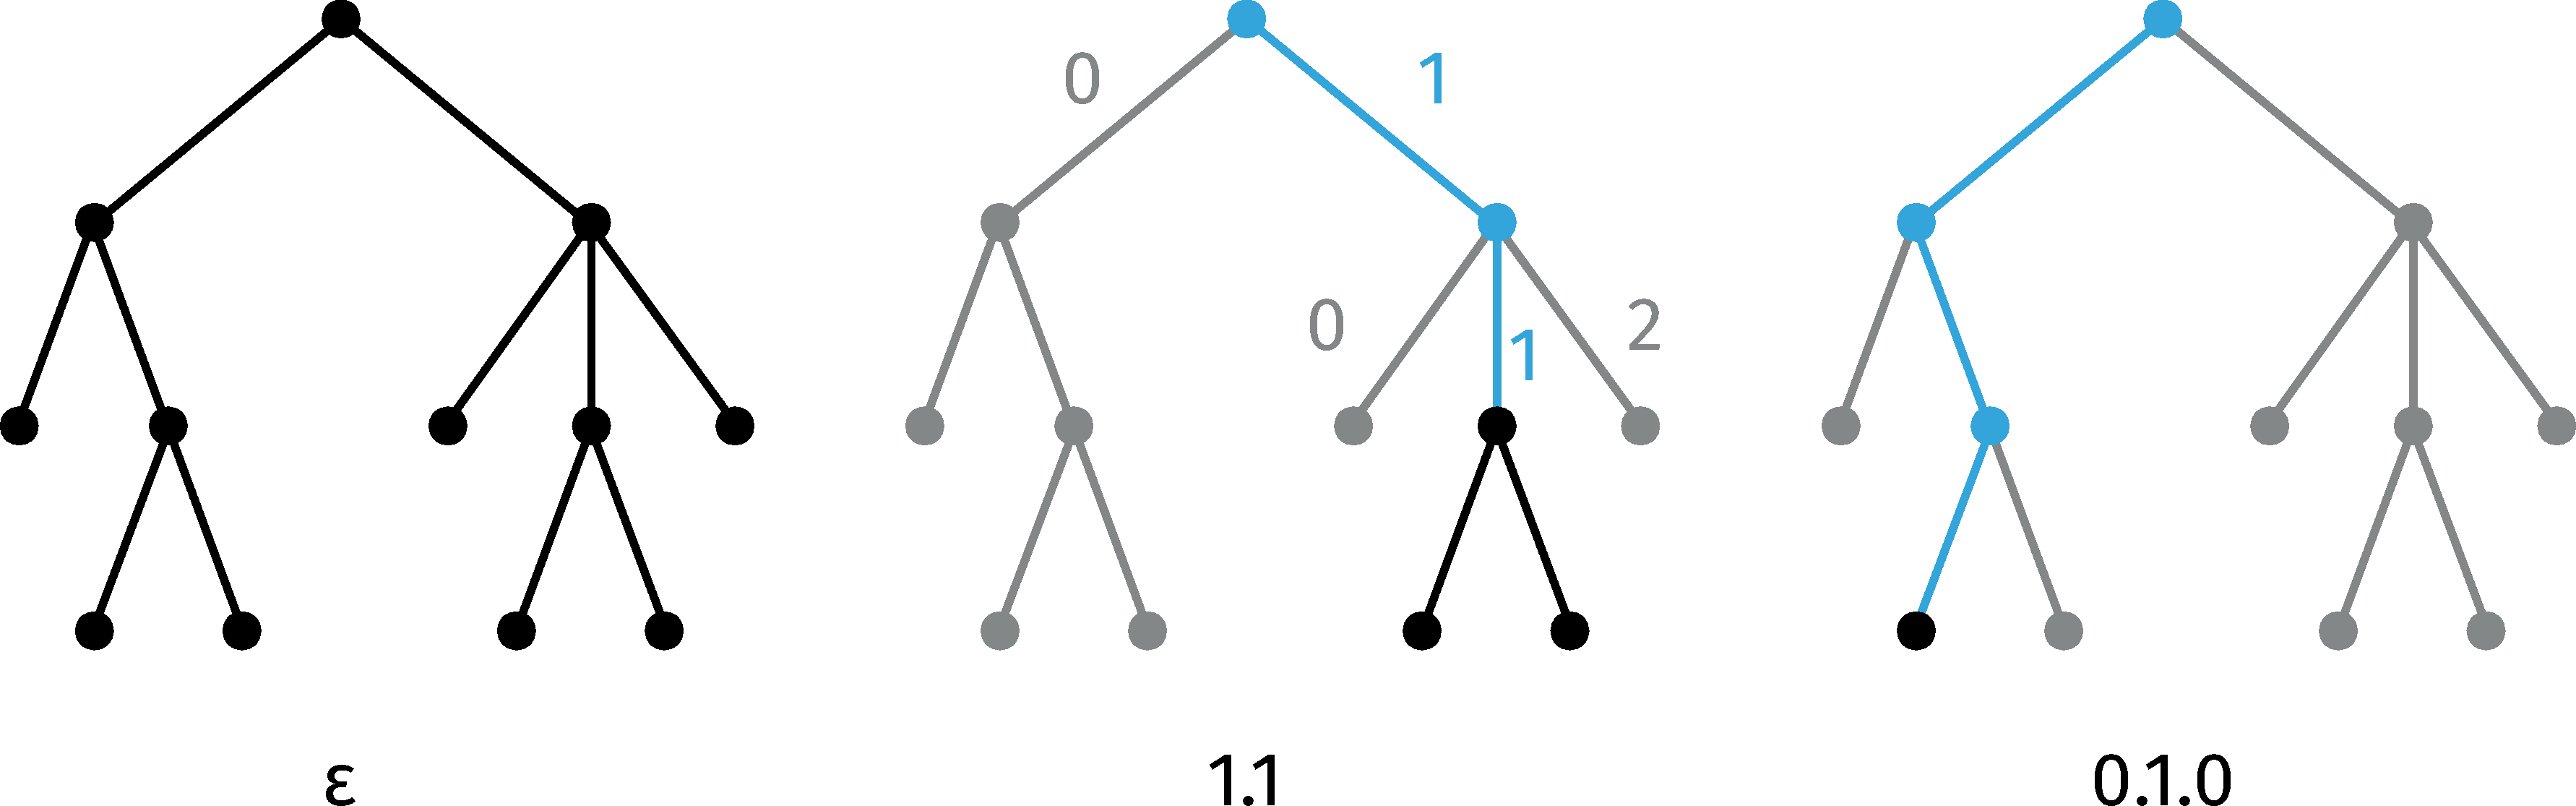
\includegraphics[width=0.9\textwidth]{tree-position.pdf}
\end{figure}

Now, terms are a special kind of tree so we can do something similar.
There are many ways to represent positions: for instance in the example above
the position \(0.3\) doesn't correspond to anything, so is it still considered
a position, only an \emph{invalid} one? Or should all expressable positions
be valid?

My approach is a bit in between, I constrain the syntax of choices a bit more
than this, but they are not necessarily valid.
Basically choices are defined inductively, with several constructors for each
of the constructs of the syntax: for instance, applications will have two
corresponding choices, one for the applicant, one for the argument.
\marginnote[1cm]{
  \mintinline{coq}{app_l} corresponds to going left under an application
  while \mintinline{coq}{app_r} corresponds to going right.
}
\begin{minted}{coq}
Inductive choice :=
| app_l
| app_r
| case_p
| case_c
| case_brs (n : nat)
| proj_c
| fix_mfix_ty (n : nat)
| fix_mfix_bd (n : nat)
| lam_ty
| lam_tm
| prod_l
| prod_r
| let_bd
| let_ty
| let_in.
\end{minted}

A position is just a list of choices.
\begin{minted}{coq}
Definition position := list choice.
\end{minted}

Now as I already said, these are not necessarily valid positions, for this
we define a function which verifies if a given position is valid in a given
term.
\marginnote[1cm]{
  It shouldn't feel too surprising, the empty position is always valid,
  and otherwise, the head choice should match the structure of the term.
  There are some trickier cases for pattern-matching and fixed-points because
  they involve lists of terms but it's still pretty natural.
}
\begin{minted}{coq}
Fixpoint validpos t (p : position) {struct p} :=
  match p with
  | [] => true
  | c :: p =>
    match c, t with
    | app_l, tApp u v => validpos u p
    | app_r, tApp u v => validpos v p
    | case_p, tCase indn pr c brs => validpos pr p
    | case_c, tCase indn pr c brs => validpos c p
    | case_brs n, tCase indn pr c brs =>
        match nth_error brs n with
        | Some (_, br) => validpos br p
        | None => false
        end
    | proj_c, tProj pr c => validpos c p
    | fix_mfix_ty n, tFix mfix idx =>
        match nth_error mfix n with
        | Some d => validpos d.(dtype) p
        | None => false
        end
    | fix_mfix_bd n, tFix mfix idx =>
        match nth_error mfix n with
        | Some d => validpos d.(dbody) p
        | None => false
        end
    | lam_ty, tLambda na A t => validpos A p
    | lam_tm, tLambda na A t => validpos t p
    | prod_l, tProd na A B => validpos A p
    | prod_r, tProd na A B => validpos B p
    | let_bd, tLetIn na b B t => validpos b p
    | let_ty, tLetIn na b B t => validpos B p
    | let_in, tLetIn na b B t => validpos t p
    | _, _ => false
    end
  end.
\end{minted}
This function might serve as a specification for the positions.

Finally we can define a type of valid positions in a term using a subset type.
\begin{minted}{coq}
Definition pos (t : term) :=
  { p : position | validpos t p = true }.
\end{minted}

For instance \mintinline{coq}{[ app_l ; let_in ]} is valid position in term
\begin{minted}{coq}
  tApp (tLetIn na b B t) u
\end{minted}
which represents the term \mintinline{coq}{(let na := b : B in t) u}
and points to subterm \mintinline{coq}{t}.

We can also define a function to access the subterm at a given position.
\marginnote[4cm]{
  The \mintinline{coq}{tRel 0} case is in an impossible branch when the position
  is valid, but for simplicity, the function is defined for any position.
  Otherwise we would have to carry the proof that it is valid everywhere.
}
\begin{minted}{coq}
Fixpoint atpos t (p : position) {struct p} : term :=
  match p with
  | [] => t
  | c :: p =>
    match c, t with
    | app_l, tApp u v => atpos u p
    | app_r, tApp u v => atpos v p
    | case_p, tCase indn pr c brs => atpos pr p
    | case_c, tCase indn pr c brs => atpos c p
    | case_brs n, tCase indn pr c brs =>
        match nth_error brs n with
        | Some (_, br) => atpos br p
        | None => tRel 0
        end
    | proj_c, tProj pr c => atpos c p
    | fix_mfix_ty n, tFix mfix idx =>
        match nth_error mfix n with
        | Some d => atpos d.(dtype) p
        | None => tRel 0
        end
    | fix_mfix_bd n, tFix mfix idx =>
        match nth_error mfix n with
        | Some d => atpos d.(dbody) p
        | None => tRel 0
        end
    | lam_ty, tLambda na A t => atpos A p
    | lam_tm, tLambda na A t => atpos t p
    | prod_l, tProd na A B => atpos A p
    | prod_r, tProd na A B => atpos B p
    | let_bd, tLetIn na b B t => atpos b p
    | let_ty, tLetIn na b B t => atpos B p
    | let_in, tLetIn na b B t => atpos t p
    | _, _ => tRel 0
    end
  end.
\end{minted}

Positions let you go deep inside a term, forgetting about its surrounding;
surrounding which can be recorded using stacks.

\section{Stacks}

My use of the term \emph{stack} might be an abuse as it's probably a
generalisation of it and might be better called an evaluation environment
or context; I will stick to \emph{stack} anyway.
The main reason behind the name is that it's not presented as a term with a hole
but rather as a succession of terms with a hole that stack on top of each other.

If you take the following example,
\[
  \stack{f\ \stack{\stack{(\lambda x. \stack{t})}\ u}}
\]
you are considering term \(t\) against the stack
\[
  \stack{f\ \stack{\stack{(\lambda x. \shole)}\ u}}
\]

It can be decomposed into
\marginnote[1cm]{
  \(\varepsilon\) represents the empty stack.
}
\[
  \stack{\lambda x. \shole} :: \stack{\shole\ u} :: \stack{f\ \shole}
  :: \varepsilon
\]
meaning that the term will first be put under an abstraction, the result of this
applied to \(u\) and the whole given as an argument to \(f\).
This notion will prove particularly useful when considering the reduction
machine in \nrefch{coq-reduction}, indeed the stack is way to remember the
surrounding term when focusing on a subterm, once it has reached a normal form,
we can use the stack as a \emph{continuation}.

You can see the process step by step in the following example.
\marginnote[2cm]{
  I use \(\red_\beta\) to denote the cases where a \emph{real} reduction
  happens and the focused term (a \(\lambda\)-abstraction) consumes its
  argument; the other cases are \emph{focusing}, \ie pushing some term with
  hole on the stack.
}
\[
  \begin{array}{lc}
    \stack{
      (
        (\lambda x.\ x\ u)\
        (\lambda y.\ y)
      ) \ v
    } & \red \\[0.2cm]
    \stack{
      \stack{(
        (\lambda x.\ x\ u)\
        (\lambda y.\ y)
      )} \ v
    } & \red \\[0.3cm]
    \stack{
      \stack{(
        \stack{(\lambda x.\ x\ u)}\
        (\lambda y.\ y)
      )} \ v
    } & \red_\beta \\[0.4cm]
    \stack{
      \stack{(
        (\lambda y.\ y)\ u
      )} \ v
    } & \red \\[0.3cm]
    \stack{
      \stack{(
        \stack{(\lambda y.\ y)}\ u
      )} \ v
    } & \red_\beta \\[0.4cm]
    \stack{
      \stack{u} \ v
    }
  \end{array}
\]

\marginnote{
  In the formalism above, \(\vscmd{t}{\stack{\shole\ u} :: \varepsilon}\)
  corresponds to \(\stack{\stack{t}\ u}\). I am simply now making explicit
  the separation betwee the focused term and the stack.
}
The intesting bit is that the focused term still interacts with the stack.
To see clearer we can use the notation \(\vscmd{t}{\pi}\) representing
term \(t\) \emph{against} stack \(\pi\). From this we can write the following
reduction rules that together correspond to \(\beta\)-reduction.

\marginnote[0.5cm]{
  \(\beta\)-reduction now happens in two steps:
  \(
    \vscmd{(\lambda x.\ t)\ u}{\pi} \red
    \vscmd{\lambda x.\ t}{\stack{\shole\ u} :: \pi} \red
    \vscmd{t[x \sto u]}{\pi}
  \)
}
\[
  \begin{array}{lcl}
    \vscmd{u \ v}{\pi} &\red& \vscmd{u}{\stack{\shole\ v} :: \pi} \\
    \vscmd{\lambda x.\ t}{\stack{\shole\ u} :: \pi}
    &\red& \vscmd{t[x \sto u]}{\pi}
  \end{array}
\]

\section{Positions induced by stacks}

\section{Ordering positions}

\todo{Should orders on positions be introduced here?
Maybe as a third section? Or maybe in reduction? We can also just talk about
the order in general, and saying that some stuff can be unspecified?}